%% Copyright 2007 Ulf Lindgren
%
% Ce document peut être distribué et/ou modifié sous les conditions définies 
% par la LaTeX Project Public License (LPPL), soit en version 1.3, soit (à 
% votre choix) en toute version ultérieure.
% La dernière version de cette license est à l'adresse :
%   http://www.latex-project.org/lppl.txt
% et la version 1.3 et les suivantes se retrouvent dans toutes les 
% distributions de LaTeX dès la version 2005/12/01.
%
% Ce document a le statut de maintenance LPPL "maintenu".
%
% Le mainteneur actuel de ce document est Ulf Lindgren.
%
% Ce document consiste en l'ensemble des fichiers listés dans le fichier
% manifest.txt.
%
%% Cette déclaration a été ajoutée le 10/12/2010 par Clea F. Ress suite à
%% la correspondance entre Ulf Lindgren et Karl Berry sur le sujet des 
%% licences.

\documentclass{report}

  \usepackage[body={16cm,23cm}]{geometry} % Pour remplacer les réglages manuels
  \usepackage[T1]{fontenc}
  \usepackage[inputenc,babel]{translatex-fr}
  \usepackage{xcolor}
  \usepackage{graphicx}
  \usepackage[Lenny]{fncychap}
  \usepackage{lettrine} % Pour remplacer ydrop qui ne donne pas les résultats attendus.

  \newcommand{\sk}{\vspace{0.2 cm}}
  \newcommand{\A}[1]{{$\backslash${\tt #1}}}
  \newcommand{\nsp}{\mbox{\hspace{-1 cm}}}
  \title{L'extension FncyChap\\V1.34}
  \author{Ulf A. Lindgren}
  \date{}

\begin{document}
  \maketitle
  \tableofcontents
  \chapter{Description de l'extension}
    \lettrine[findent=0.2em,nindent=0em,realheight=true]{L'}{extension} 
    \textsl{fncychap} a été écrite pour que des titres de chapitre puissent
    être altérés rapidement mais aussi pour que je puisse en apprendre plus sur
    \TeX{} et \LaTeX{}. Je ne sais pas d'ailleurs pas si cette extension est 
    écrite de façon adéquate : si quelqu'un lit cette documentation et
    essaye \textsl{fncychap}, je lui serais donc reconnaissant pour tout retour 
    d'expérience. Cela m'aidera à monter en compétence dans l'écriture de 
    commandes. 
 
    Dans toute publication, il est essentiel de se rappeler que la cohérence
    joue un rôle important. Avec cette extension, il est possible de modifier 
    l'apparence de chaque chapitre séparément dans un document. Mais ce
    n'est guère souhaitable pour garder son document sobre et cohérent.

    \section{Chargement et utilisation simple}
    Cette extension est chargée en saisissant la ligne suivante en 
    préambule.\sk\\    
    \nsp\fbox{\A{usepackage}[{\em style}]\{{\em fncychap}\}}\sk\\    
    Si l'option \emph{style} est omise alors la définition par défaut des 
    chapitres est utilisée. À l'origine, il existait six styles de chapitres
    prédéfinis, à savoir \emph{Sonny, Lenny, Glenn, Conny, Rejne} et 
    \emph{Bjarne}. Ces noms correspondent à des prénoms suédois, presque 
    sûrement à l'image de la pratique d'IKEA\footnote{Marque déposée par Ingvar
    Kamprad Elmtaryd Agunnaryd.}. Chacun de ces styles dispose d'une 
    configuration par défaut et, si elle est suffisante, l'adaptation du
    document s'arrête là.

    Dans la version présente de \textsl{fncychap}, deux styles additionnels
    ont été ajoutés. Le premier se nomme \emph{PetersLenny}, d'après le nom de
    son auteur Peter Osborn. Ce style se base sur celui de \emph{Lenny} : Peter
    a finement ajusté la taille des filets pour chacun des chapitres numérotés
    (jusqu'à 20) et chacune des annexes (jusqu'à Z). Le second style a été 
    défini par Jean-Marc François et il l'a nommé \textsl{Bjornstrup}.

    À l'origine, \textsl{fncychap} ne dépendait d'aucune autre extension. 
    Cependant, pour le style \emph{Lenny}, une fonte postscript est utilisée
    par défaut ; ceci reste cependant facilement modifiable. J'encourage ici 
    l'utilisation de cette fonte postscript par défaut car elle est 
    très largement redimensionnable, ce qui rend \emph{Lenny} 
    très agréable. Dans la version actuelle, si le style \textsl{Bjornstrup}
    de Jean-Marc est utilisé, l'extension \textsl{color} de la distribution de
    base sera chargée. 
    
  \chapter{Nouvelles commandes}
    \lettrine[findent=0.2em,nindent=0em,realheight=true]{E}{n} parallèle des 
    styles de chapitre, quelques commandes additionnelles sont mises à 
    disposition afin de créer des titres de chapitre personnalisés.
    Les commandes vont être décrites les unes à la suite des autres. Chaque
    commande est encadrée et placée sur une ligne séparée. Commençons donc 
    ces descriptions.\sk\\
    \nsp\fbox{\A{mghrulefill}\{{\em épaisseur}\}}\sk\\
    La commande ci-dessus est une version plus générale de la commande
    \A{hrulefill} dans le sens où l'épaisseur du filet peut être spécifiée.
    Cette commande est fournie pour décorer les titres de chapitre. Un
    titre se divise en deux parties. La première comprend \A{@chapapp} 
    contenant le texte \og Chapter \fg{}\footnote{N.D.T. : avec le chargement
    de \textsl{babel} combiné à son option \texttt{french}, ce texte est 
    \og Chapitre \fg{}.} ainsi que \A{thechapter} contenant le numéro du
    chapitre. La seconde partie est le titre du chapitre proprement dit, donné
    par l'utilisateur. À partir d'ici, \A{@chapapp} et \A{thechapter} seront
    respectivement nommés nom du chapitre et numéro du chapitre. Le titre
    donné par l'utilisateur sera nommé titre du chapitre.

    \section{Vers la personnalisation du titre de chapitre}
    \label{sec:TW}
    Noms, numéros et titres de chapitre peuvent être changés simplement. 
    Introduisons tout d'abord les deux commandes suivantes :\sk\\
    \nsp\fbox{\A{ChNameUpperCase}} et \fbox{\A{ChNameLowerCase}}\sk\\
    qui passent respectivement le nom du chapitre en lettres majuscules
    (\emph{uppercase}) ou en lettres minuscules (\emph{lowercase}). Un
    cas particulier est ajouté pour le nom du chapitre, à savoir\sk\\
    \nsp\fbox{\A{ChNameAsIs}}\sk\\
    qui affiche le format par défaut. Trois commandes similaires existent pour
    le titre du chapitre \sk\\
    \nsp\fbox{\A{ChTitleUpperCase}}, \fbox{\A{ChTitleLowerCase}} et
      \fbox{\A{ChTitleAsIs}}\ .\sk\\
    L'épaisseur du filet des styles de chapitre prédéfinis est modifiable
    par la commande\sk\\
    \nsp\fbox{\A{ChRuleWidth}\{{\em épaisseur}\}}\sk\\
    en gardant en tête que la \emph{épaisseur} doit avoir une unité, par 
    exemple \emph{pt}, \emph{mm}, etc. Les éléments liés aux polices de
    caractères tels que la police, son corps ou sa graisse peuvent être
    transmis par les commandes\sk\\
    \nsp\fbox{\A{ChNameVar}\{{\em argument}\}}, \fbox{\A{ChNumVar}\{{\em 
    argument}\}} et \fbox{\A{ChTitleVar}\{{\em argument}\}}\sk\\
    liées respectivement au nom, au numéro et au titre du chapitre. 
    L'\emph{argument} de ces fonctions peut être par exemple 
    \mbox{\A{ChNameVar}\{\A{huge}\A{rm}\A{centering}\}}.


  \chapter{Aperçu des styles de chapitre}
    \lettrine[findent=0.2em,nindent=0em,realheight=true]{L}{es} styles de 
    chapitre ont tous des paramétrages par défaut pour chacune des commandes
    décrites en section~\ref{sec:TW}. Aussi, ils peuvent être changés
    en recourant à ces commandes. Notez que si \A{centering} ou autre sont 
    utilisés pour mettre en forme le titre de chapitre, cela peut conduire
    à des résultats affreux. Le style de chapitre \emph{Bjarne} contient 
    une commande complémentaire\sk\\
    \nsp\fbox{\A{TheAlphaChapter}}\sk\\
    qui écrit le numéro du chapitre en utilisant les mots équivalents. 
    \A{TheAlphaChapter} peut écrire les nombres de \emph{ZERO} à 
    \emph{NINETYNINE}\footnote{N.D.T. : voir l'annexe \ref{french} pour une 
    redéfinition qui permette de remplacer les termes anglais par des termes
    français.}.
    
    Les styles prédéfinis sont ici présentés en compagnie de leur paramétrage 
    par défaut. Les versions \A{chapter} (dite ci-après \og normale \fg{}) et
    \A{chapter*} (dite \og étoilée \fg{}) sont toutes deux illustrées.

    \section{Le style de chapitre Sonny}
    Les paramètres par défaut sont les suivants :
    {\small\begin{verbatim}  
     \ChNameVar{\Large\sf}  \ChNumVar{\Huge}  \ChTitleVar{\Large\sf}
     \ChRuleWidth{0.5pt}    \ChNameUpperCase
    \end{verbatim}}    
    \begin{figure}[h]
      \begin{minipage}{7 cm}
        \label{fig:Sonnys}
        \centerline{\color{gray!25}\fbox{\includegraphics[height=6cm]{Sonnys.eps}}} 
        \caption{Style Sonny \og étoilé \fg{}}
      \end{minipage}\hfill
      \begin{minipage}{7 cm}
        \label{fig:Sonny}
        \centerline{\color{gray!25}\fbox{\includegraphics[height=6cm]{Sonny.eps}}}
        \caption{Style Sonny  \og normal \fg{}}
      \end{minipage}\hfill
    \end{figure}    
    
    \section{Le style de chapitre Lenny}
    Les paramètres par défaut sont les suivants :
    {\small\begin{verbatim}
     \ChNameVar{\fontsize{14}{16}\usefont{OT1}{phv}{m}{n}\selectfont}
     \ChNumVar{\fontsize{60}{62}\usefont{OT1}{ptm}{m}{n}\selectfont}
     \ChTitleVar{\Huge\bfseries\rm}  \ChRuleWidth{1pt}
    \end{verbatim}}
    \begin{figure}[h]
      \begin{minipage}{7 cm}
        \centerline{\color{gray!25}\fbox{\includegraphics[height=6cm]{Lennys.eps}}} 
        \caption{Style Lenny \og étoilé \fg{}}
      \end{minipage}\hfill
      \begin{minipage}{7 cm}
        \centerline{\color{gray!25}\fbox{\includegraphics[height=6cm]{Lenny.eps}}}
        \caption{Style Lenny \og normal \fg{}}
      \end{minipage}\hfill
    \end{figure}
    \textbf{Note :} une version alternative de ce style, nommée 
    \textsl{PetersLenny}, existe.

    \section{Le style de chapitre Glenn}
    Les paramètres par défaut sont les suivants :
    {\small\begin{verbatim}
     \ChNameVar{\bfseries\Large\sf}  \ChNumVar{\Huge}  \ChTitleVar{\bfseries\Large\rm}, 
     \ChRuleWidth{1pt}               \ChNameUpperCase  \ChTitleUpperCase
    \end{verbatim}}
    \begin{figure}[h]
      \begin{minipage}{7 cm}
        \centerline{\color{gray!25}\fbox{\includegraphics[height=6cm]{Glenns.eps}}}
        \caption{Style Glenn \og étoilé \fg{}}
      \end{minipage}\hfill
      \begin{minipage}{7 cm}
        \centerline{\color{gray!25}\fbox{\includegraphics[height=6cm]{Glenn.eps}}}
        \caption{Style Glenn \og normal \fg{}}
      \end{minipage}\hfill
    \end{figure}

    \section{Le style de chapitre Conny}
    Les paramètres par défaut sont les suivants :
    {\small\begin{verbatim}
     \ChNameUpperCase     \ChTitleUpperCase    \ChNameVar{\centering\Huge\rm\bfseries}
     \ChNumVar{\Huge}     \ChRuleWidth{2pt}    \ChTitleVar{\centering\Huge\rm}
    \end{verbatim}}
    \begin{figure}[h]
      \begin{minipage}{7 cm}
        \centerline{\color{gray!25}\fbox{\includegraphics[height=6cm]{Connys.eps}}}
        \caption{Style Conny \og étoilé \fg{}}
      \end{minipage}\hfill
      \begin{minipage}{7 cm}
        \centerline{\color{gray!25}\fbox{\includegraphics[height=6cm]{Conny.eps}}}
        \caption{Style Conny \og normal \fg{}}
      \end{minipage}\hfill
    \end{figure}

    \section{Le style de chapitre Rejne}
    Les paramètres par défaut sont les suivants :
    {\small\begin{verbatim}  
     \ChNameVar{\centering\Huge\rm\bfseries} \ChNumVar{\Huge}  \ChTitleVar{\centering\Huge\rm}
     \ChNameUpperCase                        \ChTitleUpperCase \ChRuleWidth{1pt}
    \end{verbatim}}
    \begin{figure}[h]
      \begin{minipage}{7 cm}
        \centerline{\color{gray!25}\fbox{\includegraphics[height=6cm]{Rejnes.eps}}}
        \caption{Style Rejne \og étoilé \fg{}}
      \end{minipage}\hfill
      \begin{minipage}{7 cm}
        \centerline{\color{gray!25}\fbox{\includegraphics[height=6cm]{Rejne.eps}}}
        \caption{Style Rejne \og normal \fg{}}
      \end{minipage}\hfill
    \end{figure}

    \section{Le style de chapitre Bjarne}
    Les paramètres par défaut sont les suivants :
    {\small\begin{verbatim}
     \ChNameUpperCase   \ChNameVar{\raggedleft\normalsize\rm}   \ChRuleWidth{1pt}
     \ChTitleUpperCase  \ChNumVar{\raggedleft \bfseries\Large} 
     \ChTitleVar{\raggedleft \Large\rm}
    \end{verbatim}}
    \begin{figure}[h]
      \begin{minipage}{7 cm}
        \centerline{\color{gray!25}\fbox{\includegraphics[height=6cm]{Bjarnes.eps}}}
        \caption{Style Bjarne \og étoilé \fg{}}
      \end{minipage}\hfill
      \begin{minipage}{7 cm}
        \centerline{\color{gray!25}\fbox{\includegraphics[height=6cm]{Bjarne.eps}}}
        \caption{Style Bjarne \og normal \fg{}}
      \end{minipage}\hfill
    \end{figure}

    \section{Le style de chapitre Bjornstrup}
    Les paramètres par défaut sont les suivants :
    {\small\begin{verbatim}
     \ChNumVar{\fontsize{76}{80}\usefont{OT1}{pzc}{m}{n}\selectfont}
     \ChTitleVar{\raggedleft\Large\sffamily\bfseries}
    \end{verbatim}}
    \begin{figure}[h]
      \begin{minipage}{7 cm}
        \centerline{\color{gray!25}\fbox{\includegraphics[height=6cm]{Bjornstrups.eps}}} 
        \caption{Style Bjornstrup \og étoilé \fg{}}
      \end{minipage}\hfill
      \begin{minipage}{7 cm}
        \centerline{\color{gray!25}\fbox{\includegraphics[height=6cm]{Bjornstrup.eps}}}
        \caption{Style Bjornstrup \og normal \fg{}}
      \end{minipage}\hfill
    \end{figure}
    \textbf{Note :} la restitution faite par YAP (visualisateur dvi de MikTeX)
    diffère de dvips dans la mesure où la boîte grise passe au premier plan et
    cache ainsi une partie du numéro de chapitre. 
    \enlargethispage{2cm}


  \chapter{Exemple simple}
    \lettrine[findent=0.2em,nindent=0em,realheight=true]{S}{i} les styles
    prédéfinis ne répondent pas à vos besoins, vous pouvez modifier les
    routines de mise en forme. Cette mise en forme est contrôlée par trois
    commandes. Il est possible de redéfinir les styles de chapitre d'origine
    en se servant de \A{secdef} et de \A{renewcommand}, voir pour cela le 
    \emph{\LaTeX{} Companion}. Cependant, au moment de la création de cette
    extension, j'ai décidé de rendre ce point plus simple. La commande\sk\\
    \nsp\fbox{\A{DOCH}}\sk\\
    met en forme le nom et le numéro du chapitre. Les commandes\sk\\
    \nsp\fbox{\A{DOTI}\{{\#1}\}} et \fbox{\A{DOTIS}\{{\#1}\}}\sk\\
    mettent en forme le titre du chapitre pour \A{chapter} et \A{chapter*} 
    respectivement.
    Afin de modifier celles-ci, vous devez les modifier dans le préambule du
    document et les encadrer avec les commandes \A{makeatletter} et 
    \A{makeatother}. En complément, certains paramètres prédéfinis peuvent être
    utilisés. Ces variables de longueur sont\sk\\
    \nsp\fbox{\A{mylen}}, \fbox{\A{myhi}}, \fbox{\A{px}}, \fbox{\A{py}}, 
      \fbox{\A{pxx}}, \fbox{\A{pyy}} et \fbox{\A{RW}}\ .\sk\\
    Notez que \A{RW} est particulière car elle est définie par \A{ChRuleWidth}.
    Les mises en forme indiquées par \A{ChNameVar}, \A{ChNumVar} et
    \A{ChTitleVar} sont stockées dans \A{CNV}, \A{CNoV} et \A{CTV}
    respectivement. Enfin, les fonctions \A{FmN}\{ \} pour le nom et
    \A{FmTi}\{ \} pour le titre agissent selon le choix fait avec 
    \A{Ch***AsIs}, \A{Ch***UpperCase} ou \A{Ch***LowerCase}. Notez que les 
    étoiles indiquent ici un texte à compléter en fonction du contexte ; voir 
    section~\ref{sec:TW}.
    
    Pour illustrer tout ceci, définissons un nouveau style de chapitre dans
    lequel le titre est centré et le nom comme le numéro de chapitre sont 
    placés dans une boîte encadrée (\A{fbox}). La commande \A{fboxrule} est 
    liée à la longueur prédéfinie \A{RW} de telle manière qu'elle soit 
    contrôlée par la commande \A{ChRuleWidth}. Essayez cet exemple :
    \begin{verbatim}
       \makeatletter
         \ChNameVar{\Large\rm}             % définition du style du nom
         \ChNumVar{\Huge}                  % définition du style du numéro
         \ChTitleVar{\Large\rm\centering}  % définition du style du titre
         \ChRuleWidth{4pt}                 % définition de RW à 4pt
         \ChNameUpperCase                  % utilisation de noms en majuscule
         \renewcommand{\DOCH}{%
           \setlength{\fboxrule}{\RW}      % définition des filets de fbox 
                                           % contrôlés par \ChRuleWidth

           \fbox{\CNV\FmN{\@chapapp}\space \CNoV\thechapter}\par\nobreak
           \vskip 40\p@}

         \renewcommand{\DOTI}[1]{%
           \CTV\FmTi{#1}\par\nobreak
           \vskip 40\p@}
         \renewcommand{\DOTIS}[1]{%
           \CTV\FmTi{#1}\par\nobreak
           \vskip 40\p@}
       \makeatother
    \end{verbatim}

    C'est tout ce qu'il y a à faire. Notez que les commandes \A{DOTI} et
    \A{DOTIS} peuvent être redéfinies n'importe où dans le document mais que 
    cela n'est pas une bonne idée. 

    Supposez enfin que vous souhaitiez utiliser la commande 
    \A{TheAlphaChapter}. Ceci peut être fait en choisissant initialement le
    style \emph{Bjarne} puis en redéfinissant \A{DOCH}, \A{DOTI} et \A{DOTIS}.


  \chapter{Historique}
    \lettrine[findent=0.2em,nindent=0em,realheight=true]{C}{e} 
    document décrit la version 1.34 dans laquelle deux nouveaux style de 
    chapitre ont été ajoutés et quelques problèmes mineurs ont été traités. 
    Ainsi, la gestion des majuscules et minuscules a été corrigée, tout comme
    un comportement erroné concernant les changements effectuées par 
    \verb+\frontmatter+, \verb+\mainmatter+ et \verb+\backmatter+.   

    Dans la version 1.33, le texte étiré du style \emph{Rejne} causait 
    d'horribles vides dans le filet vertical aligné avec le titre du texte. Un 
    problème de compatibilité avec la classe KOMA \og scrbook.cls \fg{}
    a été traité avec une redéfinition de \A{@schapter} en ligne avec celle 
    utilisée par KOMA. Ceci pourrait être problématique car cette nouvelle 
    définition diffère du coup de la définition de base. Par ailleurs, une 
    erreur d'orthographe a été corrigée.

    En version 1.3, un problème avec les annexes pour le style \emph{Bjarne} a 
    été traité. De plus, un mauvais comportement pour les commandes 
    \verb+\frontmatter+, \verb+\mainmatter+ et \verb+\backmatter+ a été
    corrigé.

    En version 1.11, une correction d'erreur de l'option \emph{Lenny} a été 
    ajoutée : un problème de boîte verticale sous-remplie (\emph{underfull
    vbox}), relevé par Diab Jerius, survenait quand l'option \emph{Lenny}
    était utilisée en conjonction avec la commande \A{section} et que la 
    section était composée à la page suivante. Cela provoquait le mauvais 
    placement d'une ligne. La solution revenait à placer le titre du chapitre
    dans une boîte.

    En version 1.1, une modification a été faite pour que l'extension  
    fonctionne bien avec la classe \emph{book}. Un problème, relevé par Olivier
    Guide, survenait en effet lorsque les styles \emph{Conny}, \emph{Rejne}, 
    \emph{Bjarne} ou \emph{Glenn} étaient utilisés en conjonction avec la 
    commande \A{tabelofcontents} de \LaTeX{}. La raison exacte de l'erreur n'a
    pas été trouvée. 

    Dans la version précédente, il n'y a pas eu de changement majeur de 
    l'extension. Cependant, le nom de l'extension a été changé afin de 
    respecter la convention DOS de nom de fichier à huit caractères. J'ai
    également reçu des retours m'informant que la version de \LaTeX{} devait
    être postérieure au 01/12/1994. Cette information a été ajoutée dans 
    l'extension de telle façon à ce qu'une version antérieure de \LaTeX{} 
    génère une alerte écrite dans le fichier journal (\emph{log}).

    Historique des versions :
      \begin{description}
        \item[1\iere\ version] 13/12/1996 FancyChapters 1.0b
        \item[2\ieme\ version] 08/01/1997 FncyChap 1.0 (changement de nom, test de 
          date de \LaTeX)
        \item[3\ieme\ version] 22/01/1997 FncyChap 1.1 (corrections d'erreurs)
        \item[4\ieme\ version] 06/04/1997 FncyChap 1.11 (corrections d'erreurs)
        \item[5\ieme\ version] 20/09/2004 FncyChap 1.3 (corrections d'erreurs)
        \item[6\ieme\ version] 09/08/2005 FncyChap 1.33 (corrections d'erreurs)
        \item[7\ieme\ version] 31/07/2007 FncyChap 1.34 (corrections d'erreurs)
      \end{description}

  \appendix
  \chapter{Numérotation en français} \label{french}

    Le code suivant\footnote{N.D.T. : cette annexe n'existe pas dans la 
    documentation originale mais elle semble assez utile dans un contexte de 
    documents francophones.} placé en préambule du document après le chargement
    de l'extension \textsl{fncychap} permet de franciser la numérotation du
    style \emph{Bjarne}. 

    Le code de l'extension est bien plus bref pour la notation anglaise. La
    langue française a cependant quelques exceptions (par exemple 
    \og quatre-vingts \fg{} avec son \og s \fg{} final) qui font que le
    parti pris ici est de lister chaque valeur sans chercher d'optimisation.

    \begin{verbatim}
      \makeatletter
      \renewcommand{\AlphaNo}{% Traitement de tous les cas de 0 à 100.
        \ifcase\number\theAlphaCnt
          \ifnum\c@chapter=0
        Z\'{E}RO\else{}\fi
        \or UN\or DEUX\or TROIS\or QUATRE\or CINQ
        \or SIX\or SEPT\or HUIT\or NEUF\or DIX
        \or ONZE\or DOUZE\or TREIZE\or QUATORZE\or QUINZE
        \or SEIZE\or DIX-SEPT\or DIX-HUIT\or DIX-NEUF\or VINGT
        \or VINGT-ET-UN\or VINGT-DEUX\or VINGT-TROIS\or VINGT-QUATRE
        \or VINGT-CINQ\or VINGT-SIX\or VINGT-SEPT\or VINGT-HUIT
        \or VINGT-NEUF\or TRENTE
        \or TRENTE-ET-UN\or TRENTE-DEUX\or TRENTE-TROIS\or TRENTE-QUATRE
        \or TRENTE-CINQ\or TRENTE-SIX\or TRENTE-SEPT\or TRENTE-HUIT
        \or TRENTE-NEUF\or QUARANTE
        \or QUARANTE-ET-UN\or QUARANTE-DEUX\or QUARANTE-TROIS
        \or QUARANTE-QUATRE\or QUARANTE-CINQ\or QUARANTE-SIX
        \or QUARANTE-SEPT\or QUARANTE-HUIT\or QUARANTE-NEUF
        \or CINQUANTE
        \or CINQUANTE-ET-UN\or CINQUANTE-DEUX\or CINQUANTE-TROIS
        \or CINQUANTE-QUATRE\or CINQUANTE-CINQ\or CINQUANTE-SIX
        \or CINQUANTE-SEPT\or CINQUANTE-HUIT\or CINQUANTE-NEUF
        \or SOIXANTE
        \or SOIXANTE-ET-UN\or SOIXANTE-DEUX\or SOIXANTE-TROIS
        \or SOIXANTE-QUATRE\or SOIXANTE-CINQ\or SOIXANTE-SIX
        \or SOIXANTE-SEPT\or SOIXANTE-HUIT\or SOIXANTE-NEUF
        \or SOIXANTE-DIX
        \or SOIXANTE-ET-ONZE\or SOIXANTE-DOUZE\or SOIXANTE-TREIZE
        \or SOIXANTE-QUATORZE\or SOIXANTE-QUINZE\or SOIXANTE-SEIZE
        \or SOIXANTE-DIX-SEPT\or SOIXANTE-DIX-HUIT\or SOIXANTE-DIX-NEUF
        \or QUATRE-VINGTS
        \or QUATRE-VINGT-UN\or QUATRE-VINGT-DEUX\or QUATRE-VINGT-TROIS
        \or QUATRE-VINGT-QUATRE\or QUATRE-VINGT-CINQ\or QUATRE-VINGT-SIX
        \or QUATRE-VINGT-SEPT\or QUATRE-VINGT-HUIT\or QUATRE-VINGT-NEUF
        \or QUATRE-VINGT-DIX
        \or QUATRE-VINGT-ONZE\or QUATRE-VINGT-DOUZE\or QUATRE-VINGT-TREIZE
        \or QUATRE-VINGT-QUATORZE\or QUATRE-VINGT-QUINZE\or QUATRE-VINGT-SEIZE
        \or QUATRE-VINGT-DIX-SEPT\or QUATRE-VINGT-DIX-HUIT
        \or QUATRE-VINGT-DIX-NEUF\or CENT\fi
        }  
      \renewcommand{\TheAlphaChapter}{% Simplification de la fonction existante
        \ifinapp 
          \thechapter
        \else
          \setcounter{AlphaCnt}{\c@chapter}
          \AlphaNo
        \fi
        }  
      \makeatother
    \end{verbatim}


\end{document}
%%% Local Variables: 
%%% mode: latex
%%% TeX-master: t
%%% End: 
